\section{Arquitectura del sistema (pipeline)}
Aquest apartat descriu l'arquitectura del sistema que s'ha desenvolupat per a l'anàlisi automàtica dels tiquets d'incidències de ciberseguretat de l'\textbf{Agència}. L'arquitectura del sistema està directament lligat a les màquines des de les quals s'han disposat propietat de l'\textbf{Agència} i al sistema que tenien en producció. L'\textbf{Agència} va posar a disposició de l'equip tres servidors idèntics per cada secció on estaran les dades i dos portàtils amb accés als servidors a través d'una VPN privada.

\begin{itemize}
     \item \textbf{Servidor 1 (OTRS):} Servidor on s'emmagatzema la base de dades d'OTRS amb els tiquets al seu interior.
     \item \textbf{Servidor 2 (Pipeline):} Servidor encarregat d'accedir als altres servidors per llegir i guardar informació i passar-la pel programa desenvolupat per resoldre el problema.
     \item \textbf{Servidor 3 (Elasticsearch):} Servidor que recull les dades processades i anonimitzades per un futur us.
\end{itemize}

\begin{itemize}
     \item \textbf{Portàtil 1 (amb GPU):} Portàtil amb la funció principal d'entrenar el model que serà utilitzat per extreure l'informació dels tiquets. Està configurat per evitar cap bretxa de dades.
     \item \textbf{Portàtil 2 (sense GPU):} Portàtil amb la capacitat d'accedir als servidors de l'\textbf{Agència} mitjançant una VPN. Té la mateixa configuració que el Portàtil 1.
\end{itemize}

\begin{figure}[H]
     \centering
     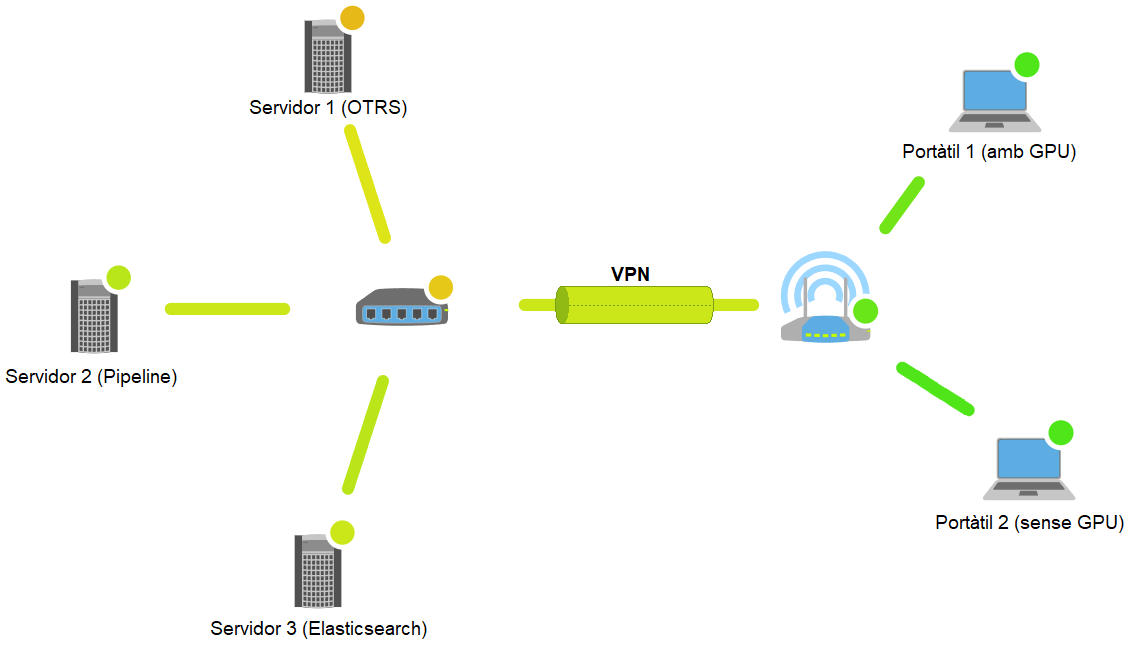
\includegraphics[width=0.8\textwidth]{network.png}
     \caption{Diagrama de la xarxa del projecte. \\ (Creació pròpia amb recursos de \textbf{yWorks})}
     \label{fig:network}
\end{figure}

El sistema consta d'una sèrie de scripts de Python que s'executen seqüencialment i duen a terme les tasques següents:

\begin{enumerate}
     \item Extreure els tiquets de la base de dades OTRS de l'\textbf{Agència}.
     \item Preprocessar el text de cada tiquet, eliminant el soroll, normalitzant el format i inserint les referències necessàries.
     \item Aplicar un model de processament del llenguatge natural (NLP) que detecta i extreu els camps rellevants de cada tiquet.
     \item Anonimitzar els camps extrets mitjançant una funció proporcionada per l'\textbf{Agència}, que substitueix les dades personals o sensibles per símbols o etiquetes genèriques.
     \item Emmagatzemar els camps anonimitzats en una base de dades Elasticsearch, que és un motor de cerca i anàlisi distribuïda.
\end{enumerate}

La figura \ref{fig:pipeline} mostra un diagrama de flux que il·lustra el funcionament del sistema.

\begin{figure}[H]
     \centering
     \vspace{1cm} % Adjust the vertical space (padding) at the top
     \setlength{\fboxsep}{5pt} % Adjust the padding
     \setlength{\fboxrule}{0pt} % Adjust the border thickness   
     \fbox{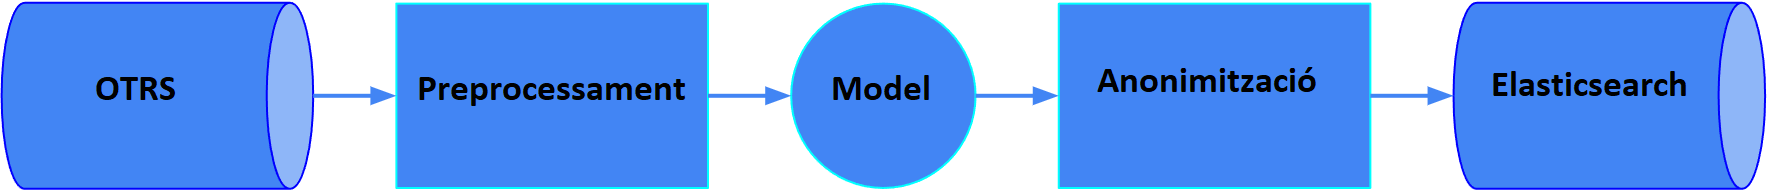
\includegraphics[width=0.8\textwidth]{pipeline.png}}
     \caption{Diagrama de flux del sistema d'anàlisi automàtica de tiquets d'incidències de ciberseguretat. \\ (Creació pròpia)}
     \label{fig:pipeline}
\end{figure}

En les següents seccions es detallen els components i les tecnologies que han sigut utilitzades a cadascuna de les etapes del \textit{pipeline}.
\subsection{Extracció de tiquets d'OTRS}
% Explicar com està configurat el OTRS
Per extreure els tiquets del Servidor OTRS de l'\textbf{Agència}, s'ha fa servir \textit{PyOTRS}, que permet accedir a les dades mitjançant peticions a través de la REST API. S'ha implementat un script de Python que utilitza la llibreria mencionada per fer les peticions i obtenir els tiquets. L'script s'encarrega d'autenticar-se amb les credencials cedides per l'\textbf{Agència}, extreure els tiquets especificats a un fitxer Excel i fer un postprocessament per aconseguir tota la informació del tiquet en un format estandarditzat i sense repeticions innecessàries. A continuació es detalla el funcionament del codi seguint l'ordre que recorren els tiquets.

\begin{enumerate}
     \item \textbf{Iniciar sessió:} Es fan unes configuracions per assegurar que els tiquets es reben amb el format esperat i mitjançant les funcions creades a OTRS. Després es crea un client amb l'adreça IP del servidor, l'usuari i la contrasenya obtingudes de l'\textbf{Agència}.
     \item \textbf{Iterar pels tiquets:} Es busca i s'obre el fitxer Excel especificat en el qual hi haurà la informació necessària dels tiquets que s'ha de processar. S'itera per la columna en la qual es troben els identificadors dels tiquets.
     \item \textbf{Llegir ID del tiquet:} Per cada fila, es llegeix l'identificador del tiquet i es crida a la següent funció.
     \item \textbf{Comprovar la utilització del tiquet:} Abans de començar a extreure els tiquets, es comprova si el tiquet en qüestió ja ha sigut extret abans. Això es fa per evitar cicles infinits amb referències cícliques dins dels tiquets. Es reinicia la llista de tiquets visitats després de cada iteració.
     \item \textbf{Extreure tiquet:} S'envia la petició al servidor OTRS mitjançant la funció \linebreak \pyth{get_ticket_by_number} de \textbf{PyOTRS}. El qual retorna un tiquet de la classe \pyth{Ticket}, molt convenientment, pel seu futur processament. En cas que el tiquet amb l'identificador especificat no existeixi, es llançarà un error informant del succés.
\end{enumerate}


\subsection{Preprocessament de tiquets}
El preprocessament dels tiquets té com a objectiu preparar el text per ser analitzat pel model de NLP. S'ha implementat un script de Python que efectua les operacions següents sobre el text de cada tiquet:
% Com s'organitza el tiquet amb els tres anteriors apartats (posar imatge/exemple)
\begin{enumerate}
     \item \textbf{Iterar pels articles:} El processament bàsic del tiquet consisteix a iterar per tots els articles del tiquet i, per cadascun d'ells unir el cos principal de l'article amb els arxius adjunts i les referències a altres tiquets. Fent això repetit per cada article fins a arribar a l'últim i evitant sempre repetir text ja mencionat anteriorment.
     \item \textbf{Processament del cos:} El primer que s'insereix és el cos principal de l'article que s'està tractant en el moment. Gràcies a una opció d'OTRS, el cos està adjuntat com un fitxer adjunt més en format HTML, permetent molta més flexibilitat a l'hora de modificar el seu contingut. Un problema que es va trobar en tots els tiquets, és que per cada article que es contesta, es torna a enviar tota la conversa fins al moment a sota. És per això que es busca l'element HTML que marca el final del tiquet (Una vora esquerra blava) i s'elimina tot el que hi ha dins. Després es converteix a text normal, s'elimina la firma (indica l'hora, lloc i altra informació irrellevant) amb una expressió regular (regex) i s'elimina tots els salts de línia sobrants.
     \item \textbf{Processament dels adjunts:} Els fitxers adjunts estan tots codificats amb la codificació \textbf{Base 64}, per tant, el primer pas és descodificar el fitxer. Després depenent del seu format es fa ús de llibreries diferents per acabar amb el fitxer en format text UTF-8. No tots els fitxers poden ser processats per extreure la seva informació, per exemple, s'ha considerat que analitzar les imatges està fora de l'àmbit d'aquest projecte i, per tant, s'ha decidit tractar els seguents formats:
          \begin{itemize}
               \item \textbf{Fitxer de text (.txt):} Per tractar els fitxers de text, simplement es pot descodificar l'arxiu amb la codificació \textbf{Base 64} i codificar el resultat binari amb la codificació UTF-8.
               \item \textbf{Fitxer de correu electrònic (.msg):} Per processar els fitxers de correu electrònic, s'ha implementat una funció que extreu el contingut de l'adjunt codificat i es descodifica a partir de la codificació \textbf{Base 64}. Les dades binàries després es codifiquen com un missatge d'Outlook amb la llibreria \pyth{extract_msg}. Amb aquest format, ara es pot llegir en format text el remitent, destinatari, subjecte i cos per recrear el correu original.
               \item \textbf{Fitxer PDF (.pdf):} Per llegir fitxers PDF, es descodifica el fitxer codificat a \textbf{Base 64} que representa un arxiu PDF i extreu el contingut de text del PDF descodificat utilitzant una biblioteca de lectura de PDF anomenada \pyth{PyPDF2}. El text extret de cada pàgina es concatena i es torna.
               \item \textbf{Document de Word (.docx):} Aquesta funció descodifica l'adjunt amb la codificació \textbf{Base 64}. El document després es descodifica en dades binàries i fa ús de la llibreria de python \pyth{docx} per carregar el fitxer .docx des de l'objecte binari. El contingut del document es pot accedir per paràgrafs i es retorna concatenant-los tots.
               \item \textbf{Antic document de Word (.doc):} Per extraure el contingut del document adjunt, el descodifica fent servir la codificació \textbf{Base 64}. Les dades binàries descodificades s'escriuen en un fitxer temporal amb extensió .doc. Després, s'utilitza l'eina externa \pyth{antiword} a través d'un subprocés per convertir el fitxer temporal .doc en text pla. Finalment, es torna el text extret com a resultat de la funció.
          \end{itemize}
     \item \textbf{Processament de les referències:} Aquesta funció intenta buscar en el text totes aquelles referències a incidències passades per intentar recrear tot el context necessari per entendre el tiquet. Es defineix un patró d'expressió regular que cerca exactament 16 dígits, que representen un número de tiquet, i cerca totes les aparicions d'aquest patró dins de l'article. Per a cada número de tiquet identificat, es recupera informació detallada sobre el tiquet referenciat utilitzant la funció \pyth{get_ticket_by_number} i indicant, en cas que sigui necessari si ja ha sigut inserida aquesta referència anteriorment.
     \item \textbf{Unir i retornar:} Finalment, s'uneixen totes les peces en un mateix text, de manera que quedarien els articles ordenats temporalment i, sota de cada article, el text dels fitxers adjunts (si han pogut ser descodificats) i els tiquets als quals es fan referència.
\end{enumerate}


\subsection{Aplicació del model}
Per aplicar el model NLP que detecta i extreu els camps rellevants de cada tiquet, s'ha fet servir la llibreria \textit{Transformers}.

\textit{Transformers} és una biblioteca de codi obert desenvolupada per \textit{Hugging Face} \cite{Hugging-Face} que ofereix models preentrenats i eines per a tasques de processament del llenguatge natural. Aquesta llibreria facilita molt l'aplicació del model i, després d'instalar totes les dependències requerides, s'utilitza la següent commanda per inicialitzar un \textit{pipeline}, que amaga tot el procés d'inferència:

\begin{python}
t2t_gen_pipe = pipeline(
     "text2text-generation",
     model='./trained_model/',
     tokenizer='google/flan-t5-base',
     device='cuda'
     )     
output_text = t2t_gen_pipe(input_ticket_str, max_new_tokens=300, beams=5)[0]['generated_text']
\end{python}

Aquest codi inicialitza un \textit{pipeline} amb la funció de generació de text a text (la tasca del model \textit{Flan-T5}), el model afinat anteriorment, el tokenitzador per defecte del model i s'indica que es faci ús dels drivers de cuda, per aprofitar tota la potència computacional de la GPU. Amb aquest \textit{pipeline}, s'indica l'entrada, el nombre màxim de tokens que pot generar el model (el model té la capacitat per parar sol, però s'indica un màxim com a mesura de seguretat) i el nombre de \textit{beams} (possibles solucions candidates, diferents unes de les altres) durant el \textit{beam search}.


\subsection{Anonimització de camps}
L'anonimització dels camps extrets té com a objectiu protegir la privadesa i la confidencialitat de les dades personals o sensibles que puguin contenir els tiquets d'incidències de ciberseguretat. Per fer-ho, s'ha utilitzat una funció proporcionada per \textbf{i2CAT}, que rep com a paràmetre el text d'un camp i torna un text anonimitzat, que substitueix les dades per símbols o etiquetes genèriques. Per exemple, si el text del camp és "Marc Vila", la funció torna "NOM COGNOM", i si el text és "192.168.1.1", la funció torna "IP PRIVADA".

La funció d'anonimització s'ha implementat en un script de Python que rep com a entrada el fitxer amb els camps extrets pel model de NLP, i torna com a sortida un altre fitxer amb els camps anonimitzats.


\subsection{Emmagatzematge del resultat}
A l'etapa final de la cadena de processament dels tiquets, l'\textbf{Agència} ha fet servir \textit{Elasticsearch} com a solució d'emmagatzematge per als camps extrets. \textit{Elasticsearch} és conegut per les seves capacitats de cerca distribuïda i en temps real, cosa que el fa eficient per gestionar i consultar grans volums de dades estructurades.

El procés comença establint una connexió amb el \textit{Servidor Elasticsearch} mitjançant una funció d'inici de sessió. Aquesta funció empra la llibreria de Python \texttt{Elasticsearch} per verificar la connectivitat amb l'adreça IP del \textbf{Servidor 2} especificada.

Un cop s'estableix una connexió amb èxit, es crida la funció per pujar els camps extrets d'un tiquet a la base de dades. La funció pren com a paràmetres un diccionari que representa els camps extrets del tiquet, la connexió Elasticsearch establerta i alguns camps necessaris com el nombre del tiquet i l'identificador.

A continuació, utilitza una funció pròpia de la llibreria \texttt{Elasticsearch} per inserir el tiquet a l'índex especificat, amb l'identificador del tiquet com a clau primària.
